\begin{frame}{Artifacts of stabilization}
  \begin{columns}
    \begin{column}{0.4\textwidth}
      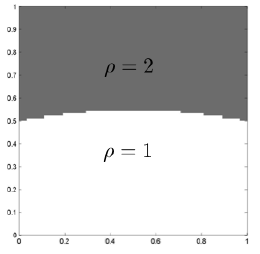
\includegraphics[width=\textwidth]{figures/Stabilization/RayleighTaylor} \\
      Rayleigh-Taylor initiation, isoviscous \\
      (Dave May and Yury Mishin)
    \end{column}
    \begin{column}{0.6\textwidth}
      $Q_2-P_{-1}$ (stable, locally conservative) \\
        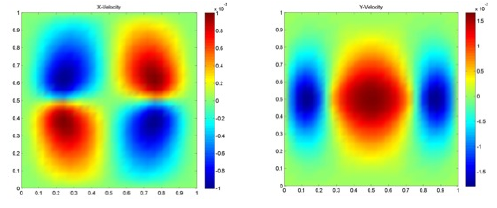
\includegraphics[width=\textwidth]{figures/Stabilization/Q2Pm1} \\
        \medskip
        $Q_1-Q_1$ (stabilized) \\
        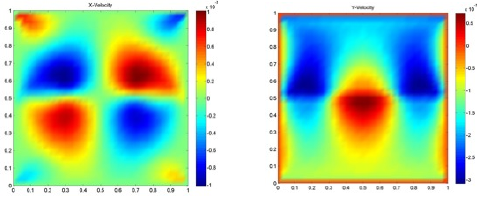
\includegraphics[width=\textwidth]{figures/Stabilization/Q1Q1stab} \\
        \vbox{\hspace{4em} $u$ \hspace{8em} $v$}
    \end{column}
  \end{columns}
\end{frame}
